% This is an AMS-LaTeX v. 1.2 File.

\documentclass{report}

%\usepackage{pscyr}
%\renewcommand{\rmdefault}{fjn}
%\renewcommand{\ttdefault}{fcr}

%\usepackage{showkeys}
\usepackage[T2A]{fontenc}
\usepackage[utf8]{inputenc}
\usepackage[english,russian]{babel}
\usepackage{expdlist}
\usepackage[dvips]{graphicx}
\usepackage{amsmath}
\usepackage{amssymb}
\usepackage{amsthm}
\usepackage{amsfonts}
\usepackage{amsxtra} 
\usepackage{sty/dbl12}
\usepackage{srcltx}
\usepackage{epsfig}
\usepackage{verbatim}
\usepackage{sty/rac}
%\usepackage[russian]{sty/ralg}
\usepackage{listings}
\usepackage{color}
\usepackage{icomma}
\usepackage{appendix} 
%\usepackage{hyperref}


%%%%%%%%%%%%%%%%%%%%%%%%%%%%%%%%%%%%%%%%%%%%%%%%%%%%%%%%%%%%%%%%%%%%%%%%%%%%%%

\renewcommand\appendixname{Приложение}

% Redefine margins and other page formatting

\setlength{\oddsidemargin}{0.5in}


% Various theorem environments. All of the following have the same numbering
% system as theorem.

\theoremstyle{plain}
\newtheorem{theorem}{Теорема}
\newtheorem{prop}[theorem]{Утверждение}
\newtheorem{corollary}[theorem]{Следствие}
\newtheorem{lemma}[theorem]{Лемма}
\newtheorem{question}[theorem]{Вопрос}
\newtheorem{conjecture}[theorem]{Гипотеза}
\newtheorem{assumption}[theorem]{Предположение}

\theoremstyle{definition}
\newtheorem{definition}[theorem]{Определение}
\newtheorem{notation}[theorem]{Обозначение}
\newtheorem{condition}[theorem]{Условие}
\newtheorem{example}[theorem]{Пример}
\newtheorem{algorithm}[theorem]{Алгоритм}
%\newtheorem{introduction}[theorem]{Introduction}

\renewcommand{\proof}{\\\textbf{Доказательство.}~}

\def\startprog{\begin{ lstlisting }[language=Java,basicstyle=\normalsize\ttfamily]}
\renewcommand{\lstlistingname}{Листинг}

%\theoremstyle{remark}
%\newtheorem{remark}[theorem]{Remark}
\include{header}
%%%%%%%%%%%%%%%%%%%%%%%%%%%%%%%%%%%%%%%%%%%%%%%%%%%%%%%%%%%%%%%%%%%%%%%%%%%%%%%

\numberwithin{theorem}{chapter}        % Numbers theorems "x.y" where x
                                        % is the section number, y is the
                                        % theorem number

%\renewcommand{\thetheorem}{\arabic{chapter}.\arabic{theorem}}

%\makeatletter                          % This sequence of commands will
%\let\c@equation\c@theorem              % incorporate equation numbering
%\makeatother                           % into the theorem numbering scheme

%\renewcommand{\theenumi}{(\roman{enumi})}

%%%%%%%%%%%%%%%%%%%%%%%%%%%%%%%%%%%%%%%%%%%%%%%%%%%%%%%%%%%%%%%%%%%%%%%%%%%%%%


%%%%%%%%%%%%%%%%%%%%%%%%%%%%%%%%%%%%%%%%%%%%%%%%%%%%%%%%%%%%%%%%%%%%%%%%%%%%%%%

%This command creates a box marked ``To Do'' around text.
%To use type \todo{  insert text here  }.

\newcommand{\todo}[1]{\vspace{5 mm}\par \noindent
\marginpar{\textsc{ToDo}}
\framebox{\begin{minipage}[c]{0.95 \textwidth}
\tt #1 \end{minipage}}\vspace{5 mm}\par}

%%%%%%%%%%%%%%%%%%%%%%%%%%%%%%%%%%%%%%%%%%%%%%%%%%%%%%%%%%%%%%%%%%%%%%%%%%%%%%%

\binoppenalty=10000
\relpenalty=10000

\begin{document}


\bibliographystyle{sty/gost71u}       % Set the bibliography style to AMS
                                % alphabetized. (Can use ``amsalpha'' or
                                % ``abbrv''instead.)

% Begin the front matter as required by Rackham dissertation guidelines

\initializefrontsections

\pagestyle{title}

\begin{center}
Санкт-Петербургский государственный университет \\ информационных технологий, механики и оптики

\vspace{2cm}

Факультет информационных технологий и программирования \\
Кафедра компьютерных технологий

\vspace{3cm}

{\Large Лебедева А. В.}

\vspace{2cm}

\vbox{\LARGE\bfseries
Статическая приоритезация поискового робота.
}

\vspace{4cm}

Дипломная работа 

\vspace{1cm}

{\Large Научный руководитель: Романенко А. А.}

\vspace{6cm}

Санкт-Петербург\\ 2013
\end{center}

\newpage

\setcounter{page}{3}
\pagestyle{plain}

%\dedicationpage{Put a dedication here}
% Dedication page

%\startacknowledgementspage
% Acknowledgements page
%{Put Acknowledgements here}

% Table of contents, list of figures, etc.
\tableofcontents
%\listoffigures


\def\t#1{\mbox{\texttt{\hbox{#1}}}}
\def\b#1{\textbf{#1}}
\def\tb#1{\t{\b{#1}}}

\def\cln#1{\t{#1}}
\def\pcn#1{\t{#1}}
\newcommand{\p}{\par Здесь будет текст...}

\def\drawfigure#1#2#3{
        \begin{figure}[H]
        \centerline{ \includegraphics{pics/#1}}
        \caption{#2}
        \label{#3}
        \end{figure}
}
\def\drawfigurex#1#2#3#4#5{
        \begin{figure}[#1]
        \centerline{ \includegraphics[#2]{#3}}
        \caption{#4}
        \label{#5}
        \end{figure}
}

% Chapters
\startthechapters
\startprefacepage

Объем информации в интернете в последнее время очень быстро растет. На данный момент число сайтов исчисляется исчисляется десятками миллиардов, а число веб-страниц --- десятками биллионов. Кроме того, информация в интернете быстро изменяется, веб-страницы обновляются все чаще. 

В связи с данными особенностями развития интернета поиск необходимой информации является очень сложной задачей для пользователя. Для упрощения этой задачи были созданы поисковые системы. 

Поисковый робот является частью поисковой системы, необходимой для ее корректного функционирования. Его задачей является перебор страниц интернета. Загруженные роботом страницы сохраняются в базу данных поисковой системы для последующих выдач в пользовательских поисковых запросах.

Чтобы удовлетворять требованиям пользователей, в поисковая система должна хранить в своей базе веб-страницы, которые будут востребованы пользователями поисковой системы. Для этого необходима стратегия отбора веб-страниц, которые поисковый робот должен скачать, и в каком порядке. Для чего необходим алгоритм ранжирования веб-страниц, который будет определять важность веб-страницы. Существует два основных подхода к ранжированию веб-страниц. Первый подход основан на анализе веб-графа. Второй --- на анализе текстовых особенностей веб-страницы, особенностей ее URL-адреса и анализе ее содержимого. 

На основе анализа веб-графа построен алгоритм приоритезации PageRank, который успешно использует поисковая система Google. Но вычисление подобного ранга для каждой страницы является очень ресурсоемкой операцией, поскольку для этого необходимо использовать информацию о всем веб-графе, размер которого велик. 

На базе графовых алгоритмах ранжирования построен ряд стратегий отбора веб-страниц. Например, OPIC \cite{OPIC}, который также является аппроксимацией вычисления PageRank. Также были разработаны алгоритмы, использующие в основе приоритезации информацию о расстоянии между страницами в веб-графе, например, FICA \cite{FICA}. 

На основе анализа статических факторов страницы был разработан алгоритм ранжирования веб-страниц FRank, описанный в работе \cite{FRank}. Но вопрос его применения к приоритезации поискового робота остается открытым, поскольку оценка важности страницы требует информации не только о URL-адресе веб-страницы, но и об ее содержимом.

Кроме того, поисковая система должна располагать актуальной информацией о состоянии веб-страниц. Для чего поисковый робот должен повторно скачивать веб-страницы, уже имеющиеся в базе поисковой системы. Здесь возникает вопрос: как часто повторно скачивать веб-страницы, и в каком порядке. Для чего необходима стратегия повторного скачивания.

Алгоритм приоритезации поискового робота представляет собой комбинацию двух стратегий: отбора веб-страниц и повторного скачивания.

В данной работе описывается разработка программы, реализующей поискового робота. Для алгоритма приоритезации кототого примененяется как анализ веб-графа, так и анализ текстовых особенностей URL-адресов веб-страниц.

% vim:filetype=tex:
\chapter{Обзор предметной области}

В данной главе приведено описание предметной области. Описаны существующие подходы к алгоритмам ранжирования веб-страниц и стратегии приоритезации поискового робота.

\section{Основные понятия}

\subsection{Интернет как граф}
\label{webgraph}

Одной из формальных моделей, с помощью которой можно представить интернет, является его представление в виде направленного графа. Вершинами в этом графе являются веб-страницы, а ребрами --- ссылки. Из вершины $u$ есть ребро в вершину $v$, если на веб-странице, соответвующей узлу $u$ есть ссылка на веб-страницу, соответствующей вершине $v$. Заметим, что данный граф является динамическим, поскольку веб-страницы часто изменяются, какие-то из них удаляются, а также создаются новые. 

\subsection{Поисковая система}

Поисковая система --- это программный комплекс, предназначенный для помощи пользователю осуществления поиска информации в интернете. Основные компоненты поисковой системы представлены на рисунке \ref{poisk}. 

\begin{figure}[h!]
\center{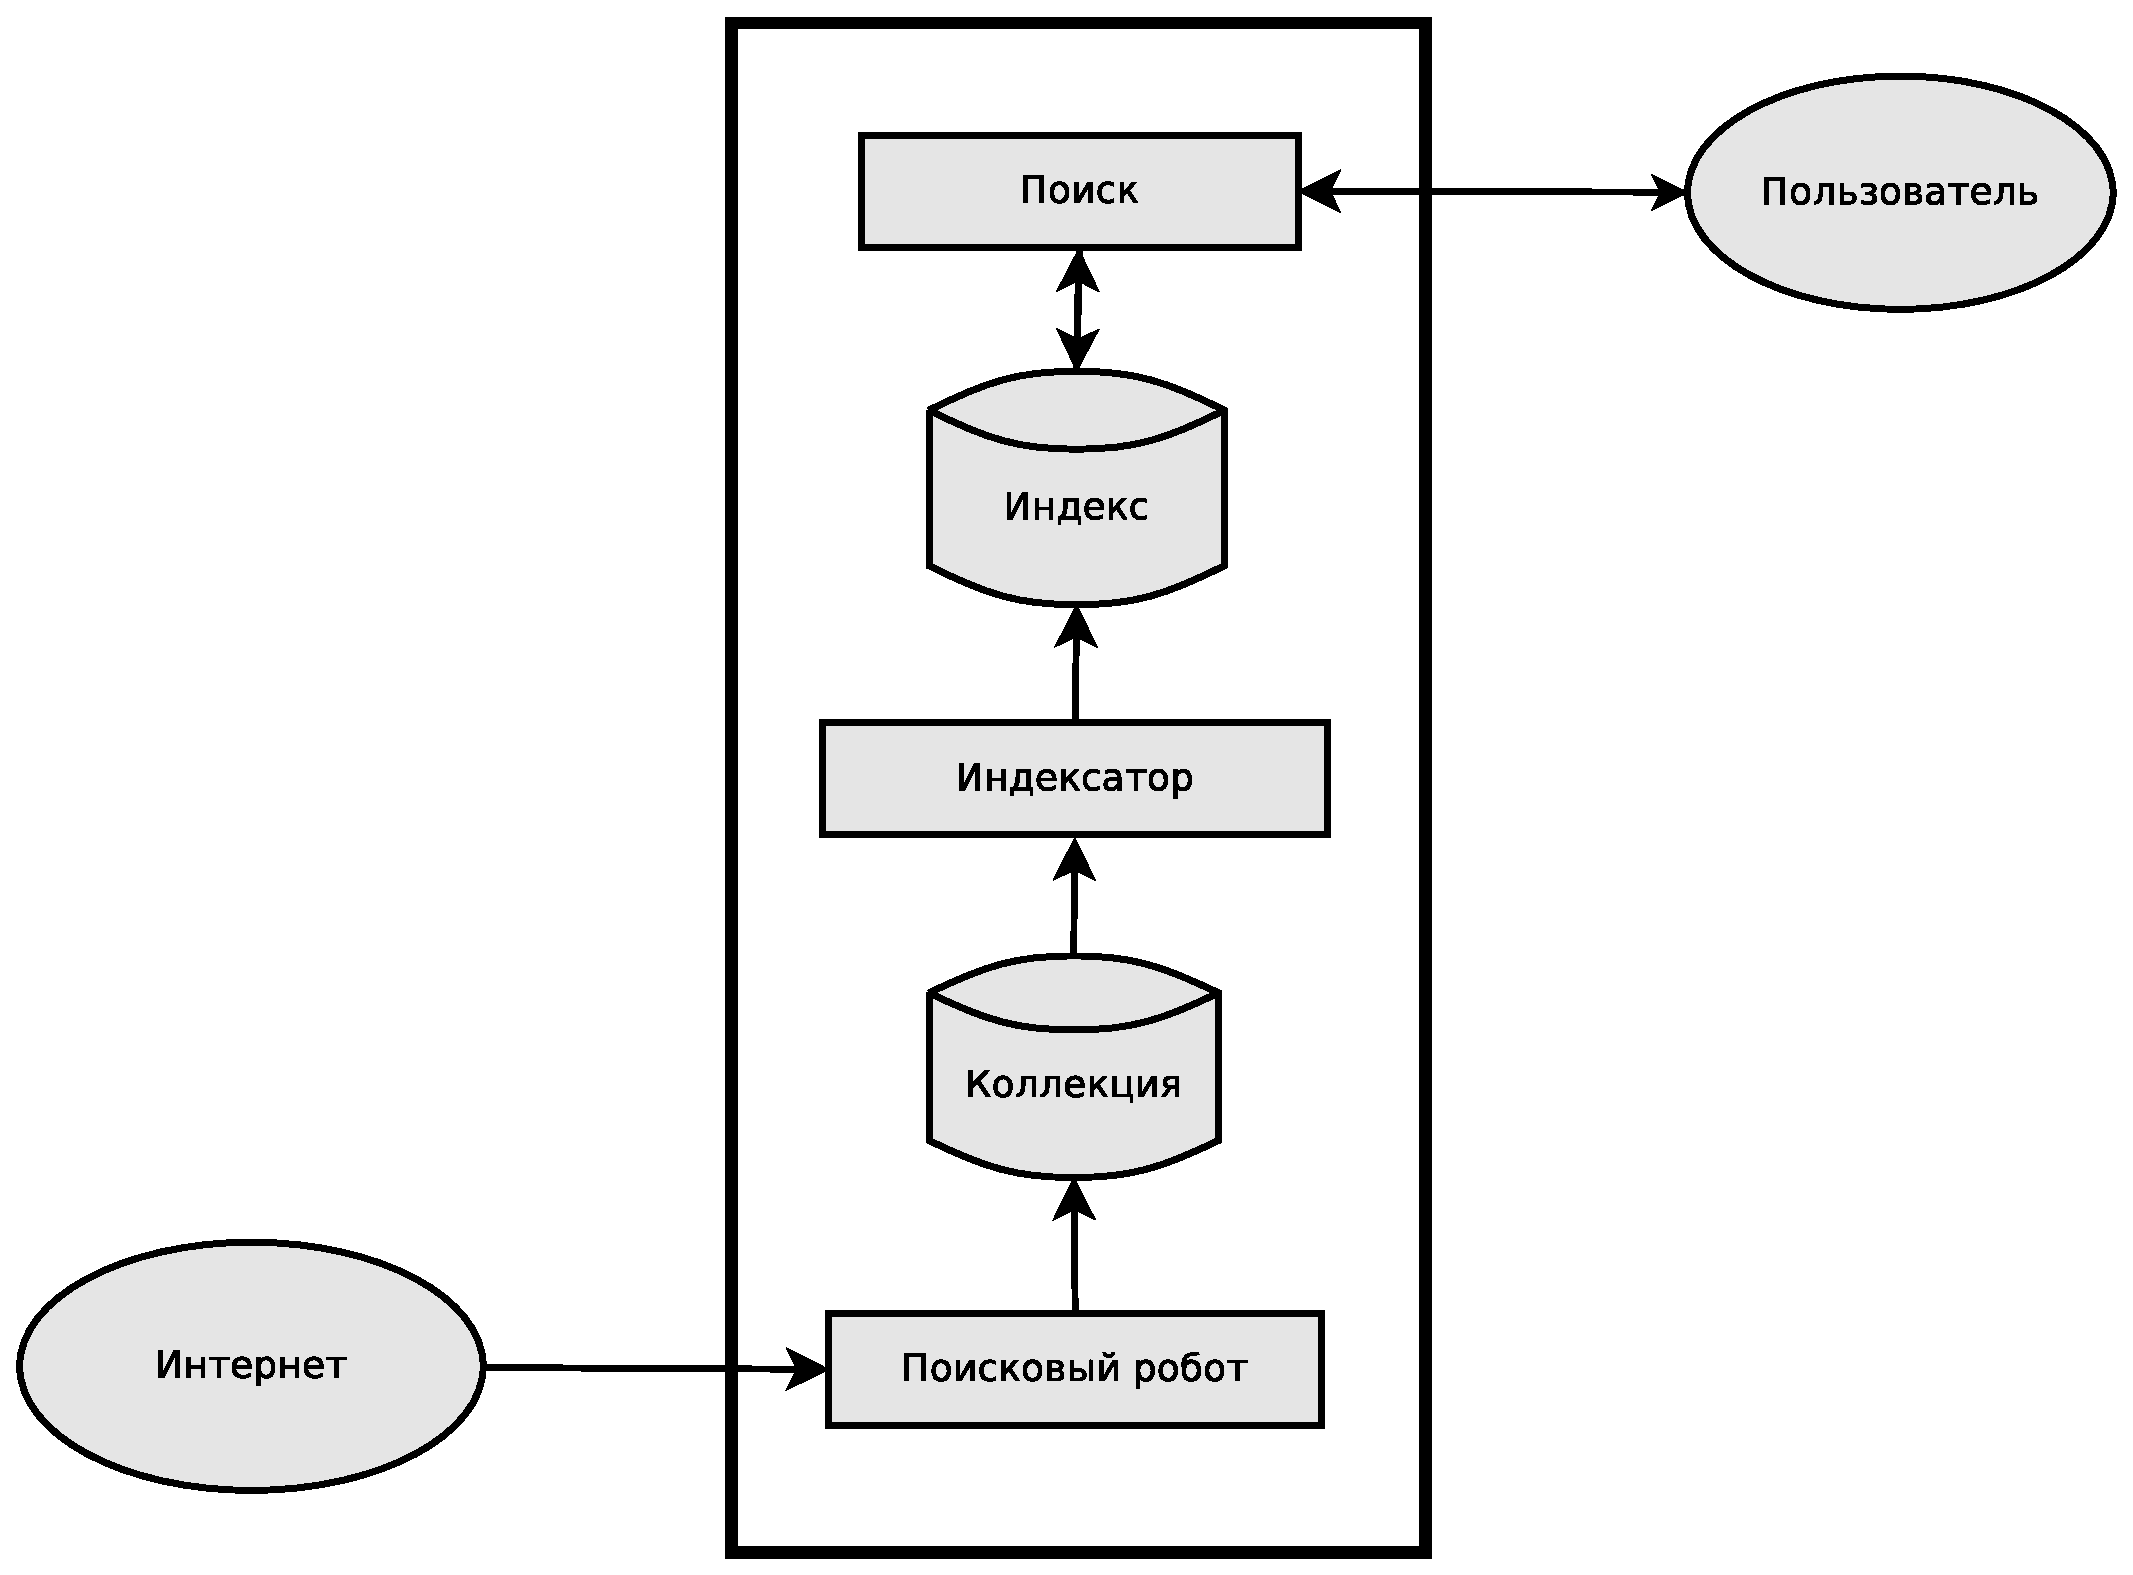
\includegraphics[width=1\linewidth]{pics/poisk.eps}}
\caption{Основные компоненты поисковой системы}
\label{poisk}
\end{figure}

Когда пользователь осуществляет информационный запрос, поисковая система формирует упорядоченное подмножество веб-страниц, хранящихся в ее индексе. Таким образом, качество работы поисковой системы во многом зависит от содержимого индекса, формирование которого осуществляется индексатором из множества веб-страниц коллекции, полученной в процессе обхода интернета, потому очень важно, чтобы в коллекции содержались важные веб-страницы, то есть веб-страницы, востребованные пользователем. Алгоритмы определения важности веб-страниц описаны в разделе \ref{ranking}. Коллекцию, в свою очередь, формирует поисковый робот. Подробное описание работы которого приведено в разделе \ref{spider}. Таким образом, поисковый робот в процессе обхода должен производить оценку страниц, и скачивать лишь важные. 

\section{Оценка важности веб-страниц}
\label{ranking}

Оценка важности веб-страницы называется рангом. Процесс получения оценки важности страницы называется ранжированием. Рассмотрим существующие методы, осуществляющие ранжирование.

\subsection{Алгоритмы ранжирования, использующие свойства веб-графа}

Данная категория алгоритмов использует представление интернета в виде графа, описанное в разделе \ref{webgraph}.

\subsubsection*{PageRank}

Метод разработан Сергеем Брином и Ларри Пейджом, основателями поисковой системы Google. Первая статья, описывающая этот алгоритм ранжирования была опубликована в 1998 году \cite{Brin}. Основная идея метода заключается в том, что страницы, чаще посещаемые в ходе случайного обхода веб-графа, имеют большую важность. 
Пусть имеется $N$ веб-страниц. Обход начинается с веб-страницы $p$, и в каждый момент времени с вероятностью $\alpha$ осуществляется переход по случайной ссылке, имеющейся на текущей странице. Также с вероятностью $1 - \alpha$ мы переходим на случайную страницу. Итоговая формула для вычисления PageRank имеет следующий вид: 
$$PageRank(p) = \frac{1 - \alpha}{N} + \alpha * \sum_{p' \in In(p)} \frac{PageRank(p')}{|Out(p')|}$$
где $In(p)$ --- множество страниц, содержащих ссылку на $p$, $Out(p')$ --- множество страниц, на которые ссылается $p'$, а $\alpha$ --- фиксированный параметр ($0 < \alpha < 1$). 

Ранжирование с использованием этого алгоритма является достаточно ресурсоемкой операцией, и требует знания о всей структуре веб-графа, что делает применение данного подхода на практике достаточно затруднительным.

\subsubsection*{HITS}

Hyperlink-Induced Topic Search (HITS) --- метод, разработанный в 1999 году Джоном Клейнбергом и описанный в работе. В отличие от \textit{PageRank}, является запросо-зависимым алгоритмом ранжирования, то есть полученные в результате анализа ссылок оценки веб-страниц зависят от конкретного поискового запроса. Базовая идея алгоритма заключается в том, что определенные веб-страницы являются \textit{посредниками} (\textit{hubs}), то есть используются как каталоги, указывающие на другие страницы, являющиеся авторитетными источниками (\textit{authorities}) или \textit{авторами} \cite{wiki_hits}, которые содержат необходимую пользователю информацию. Тогда страница, указывающая на большое количество хороших \textit{авторов}, является хорошим \textit{посредником}, и наоборот, страница, на которую ссылается много хороших \textit{посредников}, является хорошим \textit{автором}. Основываясь на этом, для каждой страницы вычисляется две оценки: оценка авторитетности и посредническая оценка. 

Для начала работы алгоритма необходимо получить множество наиболее релевантных страниц для текущего поискового запроса, называемое \textit{корневым множеством} (\textit{root set}). На его основе формируется \textit{базовое множество} (\textit{base set}), получаемое в результате добавления к \textit{корневому множеству} всех веб-страниц, связанных с ним ссылками, как исходящими, так и входящими. Все вычисления проводятся на подграфе, сформированном \textit{базовым множеством}. Основной алгоритм выполняет ряд итераций, на каждой из которых происходит обновление оценок для каждой вершины подграфа. Обновление посреднической оценки выполняется посредством суммирования оценок авторитетности каждой из вершин, на которые указывает текущая. В свою очередь, обновление авторитетной оценки осуществляется путем суммировния посреднических оценок вершин, ссылающихся на текущую. Окончательные оценки формируются после выполнения большого числа итераций алгоритма.

\subsection{Обучение ранжированию}
\label{learning_to_rank}

Алгоритмы данной категории используют методы машинного обучения для ранжирования документов. По обучающей выборке из элементов с заданным на них частичным порядком строится ранжирующая модель, которая затем используется для ранжирования новых данных. Как правило, необходимо отсортировать документы, отвечающие некоторому поисковому запросу. Элемент представляет собой пару: документ-запрос, для которой строится числовой вектор ранжирующих признаков. Признаки можно разделить на три группы:

\begin{itemize}
\item \textit{Запросо-независимые}. Зависят только от самого документа, а не от запроса. Например, \textit{PageRank} или длина документа.
\item \textit{Признаки запроса}. Зависят только от запроса. Например, число слов в запросе.
\item \textit{Запросо-зависимые}. Зависят как от документа, так и от запроса. Например, ранг \textit{HITS}, мера \textit{TF-IDF} соответствия запросу и т.д.
\end{itemize}

В статье \cite{Liu} рассмотрены существующие подходы к обучению ранжировнию и разделены на следующие категории в соответствии с форматом входных данных и функцией потерь:

\begin{itemize}
\item \textit{Поточечные подходы}. Каждому элементу сопоставляется численная оценка. Задача обучения --- по паре запрос-документ предсказать ее оценку. К ним относятся: \textit{OPRF, SLR, Pranking}.
\item \textit{Попарные подходы}. На вход подаются два документа и необходимо определить, какой из них лучше. Среди них алгоритмы: \textit{RankSVM, RankBoost, RankNet, FRank} и т.д.
\item \textit{Списочные подходы}. На вход подается сразу весь набор документов, соответвующих данному запросу, а на выходе должна получиться их перестановка. Среди них: \textit{ListNet, AdaRank, SoftRank, BayesRank} и т.д.
\end{itemize}

\section{Поисковый робот}
\label{spider}

\subsection{Общее описание}

Одним из важнейших условий функционирования поисковой системы является осуществление обхода интернета (web crawling). Его производит поисковый робот (web crawler or spider). Принцип его работы заключается в следующем. Робот хранит очередь URL-адресов веб-страниц, которые ему необходимо обойти. На момент начала обхода в ней находится некоторое исходное множество адресов. На каждой итерации робот извлекает из очереди следующий URL-адрес и скачивает веб-страницу, которая ему соответствует. Затем полученная страница обрабатывается, из нее извлекается содержимое и ссылки. Содержимое передается индексатору для последующей обработки и добавления страницы в базу поисковой системы. А URL-адреса страниц, содержащихся в ссылках, извлеченных с текущей страницы, добавляются в очередь на скачивание.

В книге \cite{Manning} сформулированы основные свойства поискового робота. Они разделены на две категории: обязательные и желательные.

\subsection{Обязательные свойства}

Обязательными свойствами поискового робота являются:
\begin{enumerate}
\item Устойчивость. 
\item Вежливость. 
\end{enumerate}

Остановимся на каждом из них подробнее.

\subsubsection*{Устойчивость}

Число страниц в интернете потециально может быть бесконечно, поскольку некоторые веб-сервера генерируют динамические веб-страницы по запросу на их создание, которым, в частности, является переход по ссылке. Таким образом, поисковый робот может зациклиться на определенном хосте, бесконечно скачивая вновь сгенерированные динамические страницы. Такой механизм называется ловушкой для роботов (spider trap). Поисковый робот должен быть устойчив к подобного рода явлениям.

\subsubsection*{Вежливость}

Для сайтов существуют явные и неявные правила поведения поискового робота при работе с ними. Эти правила регулируют частоту обращения к хосту, а также возможность доступа к его содержимому. Многие сайты имеют в корне специальный файл $robots.txt$, содержащий желательные правила поведения. Поисковый робот должен соблюдать их.

\subsection{Желательные свойства}

Желательными свойствами поискового робота являются:

\begin{enumerate}
\item Распределенность.
\item Масштабируемость.
\item Производительность и эффективность.
\item Качество.
\item Свежесть.
\item Расширяемость.
\end{enumerate}

Остановимся на каждом из них подробнее.

\subsubsection*{Распределенность}

Подразумевает возможность функционирования поискового робота одновременно на многих машинах.

\subsubsection*{Масштабируемость}

Подразумевает возможность увеличения эффективности поискового робота при увеличении ресурсов. Таких как увеличение числа машин или расширения полосы пропускания.

\subsubsection*{Производительность и эффективность}

Подразумевает эффективное использование поисковым роботом доступных ему ресурсов. 

\subsubsection*{Качество}

Желательно, чтобы поисковый робот при скачивании веб-страниц отдавал предпочтение более качественным. Для выполнения этого свойства необходима стратегия приоритезации страниц. Существующие стратегии подробнее рассмотрены в разделе \ref{algorithms}.

\subsubsection*{Свежесть}

Для хранения свежей информации о веб-страницах в базе поисковой системы необходимо, чтобы поисковый робот обходил ранее скачанные страницы с частотой, соответствующей частоте их обновления. Способы выполнения этого свойства также рассмотрены в разделе \ref{algorithms}.

\subsubsection*{Расширяемость}

Поисковый робот должен быть разработан так, чтобы имелась возможность расширения для решения новых задач. Таких как добавление новых протоколов передачи данных или новых форматов данных. 

\section{Алгоритм приоритезации поискового робота}
\label{algorithms}

Под приоритезацией подразумевается введение полного или частичного порядка на множестве веб-страниц, которое поисковый робот должен обработать. Это необходимо для того, чтобы поисковая система хранила в базе страницы, содержащие информацию, которая необходима пользователю, осуществяляющему поисковый запрос. Скачивание качественных веб-страниц осуществляется за счет применения стратегии отбора, а наличие свежей информации в базе данных поисковой системы осуществляется за счет применения той или иной стратегии повторного обхода. Объединение этих двух стратегий составляет стратегию приоритезации поискового робота. 

\subsection{Стратегии отбора}
\label{selection_strategy}

Стратегия отбора определяет, в каком порядке поисковый робот должен обрабатывать веб-страницы, URL-адреса которых были добавлены в очередь на скачивание. Для этого необходимо осуществить эвристическую оценку важности для каждой веб-страницы, являющейся кандидатом на скачивание. В книге \cite{Castillo} стратегии отбора разделены на три категории, описанные ниже.

\subsubsection*{Стратегии, не использующие дополнительную информацию}

Стратегии, отнесенные в данную категорию, используют информацию, полученную в процессе текущего обхода, и никакую более.

\textbf{Обход в ширину}. При использовании данной стратегии поисковый робот скачивает новые страницы, осуществляя обход в ширину веб-графа, начиная с главных страниц стартового множества. То есть веб-страница будет скачана тем раньше, чем раньше ссылка на нее была извлечена с какой-либо скачанной веб-страницы. В работе \cite{Najork} показано, что в проведенных экспериментах поисковый робот, использующий данную стратегию, выбирал важные страницы первыми.

\textbf{OPIC}. Данный метод описан в работе \cite{OPIC}. Этот метод также базируется на представлении веба как графа, описанному в разделе \ref{webgraph}. В начале обхода каждой странице присваивается одинаковая стоимость. После загрузки страницы ее стоимость поровну распределяется между веб-страницами, на которые она ссылается. Более высокий приоритет имеют страницы с высокой текущей стоимостью. Вычисление стоимости аппроксимирует вычисление \textit{PageRank}. 

\textbf{Количество обратных ссылок}. Данная стратегия была описана в работе \cite{Cho2}. В этом алгоритме первыми скачиваются страницы, имеющие наибольшее число входящих ссылок.

\textbf{FICA}. Метод подробно описан в статье \cite{FICA}. Алгоритм базируется на методике обучения с подкреплением, где для каждого узла веб-графа вычисляется ранг на основании расстояния между страницами.

\subsubsection*{Стратегии, использующие информацию, полученную ранее}

Стратегии данной категории используют информацию о рангах страниц, полученную в результате предыдущих обходов. При этом поисковый робот начинает обход со страниц, имеющих более высокий ранг, а ранги для страниц, найденных впервые, рассчитываются следующими способами: 

\begin{itemize}
\item Запрашивая информацию о рангах у <<оракула>>, располгающего полной информацией о веб-графе;
\item Равновероятно выбирая одно из значений рангов страниц, полученных в предыдущих обходах;
\item Назначаются нулем, то есть сначала скачиваются все страницы, известные ранее, а затем --- новые;
\item Как значение ранга страницы, указывающей на нее, деленное на число ее исходящих ссылок.
\end{itemize}

По результатам экспериментов в работе \cite{Castillo}, стратегии данной категории преимущественно превосходят стратегии, не использующие дополнительной информации. При этом лучшим является метод, запрашивающий информацию о рангах у <<оракула>>.

\subsubsection*{Стратегия с полной информацией}

К данной категории относится одна стратегия \textit{Omniscient}, использование которой подразумевает наличие <<оракула>>, который вычисляет актуальный ранг для каждой веб-страницы. Для того, чтобы выбрать страницы из очереди на скачивание, поисковый робот осуществляет запрос к <<оракулу>>, после чего выбирает страницы с наибольшим рангом. Данная стратегия быстрее всего находит важные страницы.
 
\subsection{Стратегии повторного обхода}

Стратегия повторного обхода определяет какие из уже скачанных страниц следует скачать еще раз. Оба типа стратегий описаны в работе \cite{Cho}:

\begin{itemize}
\item \textit{С одинаковой частотой}. Данная стратегия подразумевает, что веб-страницы будут скачиваться с одинаковой частотой, при этом их важность никак не будет учитываться.
\item \textit{С разными частотами}. При использовании данного типа стратегии, веб-страницы скачиваются с разными частотами. Например, с частотами, пропорциональными частотам изменения страниц.
\end{itemize}

\chapter{Предлагаемый метод}
\label{chapter_method}

В ходе работы был разработан и реализован программный модуль, реализующий поискового робота. В разделе \ref{strategy} описана предлагаемая стратегия приоритезации, а в разделе \ref{steps} описаны основные этапы алгоритма работы поискового робота.

\section{Стратегия приоритезации}
\label{strategy}

Основная идея стретегии приоритезации заключается в объединении стратегии отбора и стратегии повторного обхода. Это осуществляется посредством введения единого значения $VRank$ (visit rank). Вычисление такого ранга для веб-страницы $p$ осуществляется по следующей формуле:
$$VRank(p) = QRank(p) * RVRank(p)$$
где $QRank(p)$ --- эвристическая важность страницы, то есть ранг, характеризующий ее качество (quality rank), а $RVRank(p)$ --- ранг, характеризующий необходимость повторно скачивать веб-страницу $p$ (re-visit rank). 

Вычисление $QRank$ производится с использованием нейронной сети. Задача нейронной сети --- по URL-адресу веб-страницы получить число, имеющее смысл эвристической оценки важности страницы. Для чего на основании URL-адреса строится вектор статических особенностей. Список особенностей представлен в разделе \ref{static_features}. Нейронная сеть принимает на вход этот вектор и вычисляет ранг веб-страницы.

Для вычисления $QRank$ предлагается два метода. Первый базируется исключительно на статических особенностях URL-адреса, и для каждой веб-страницы $QRank$ вычисляется один раз при добавлении адреса в коллекцию. Второй также использует свойства веб-графа. А именно, после обработки скачананной страницы, ее $QRank$ распределяется между страницами, ссылки на которые она содержит. Таким образом, при добавлении нового URL-адреса $QRank$ считается при помощи нейронной сети, а затем он может изменятся в процессе дальнейшей работы.

Метод вычисления $RVRank$ основан на следующей идее. Заново обходить веб-страницы следует с частотой, пропорциональной частоте их изменения. Для чего для каждой страницы необходимо определить период ее изменения. Это осуществляется посредством итеративного приближения, то есть уточнения значения периода измения страницы при каждом ее скачивании.

Кроме того, следует учитывать, что существуют динамические страницы, которые генерируются заново при переходе по URL-адресу. Динамические страницы не следует скачивать бесконечно часто. Это осуществляется, во-первых, за счет вероятного небольшого значения $QRank$ таких страниц, а во-вторых, путем введения нижней границы для значения периода изменения.

\section{Этапы алгоритма}
\label{steps}

Основные компоненты разработанного поискового робота представлены на рисунке \ref{architecture}.

\begin{figure}[h!]
\center{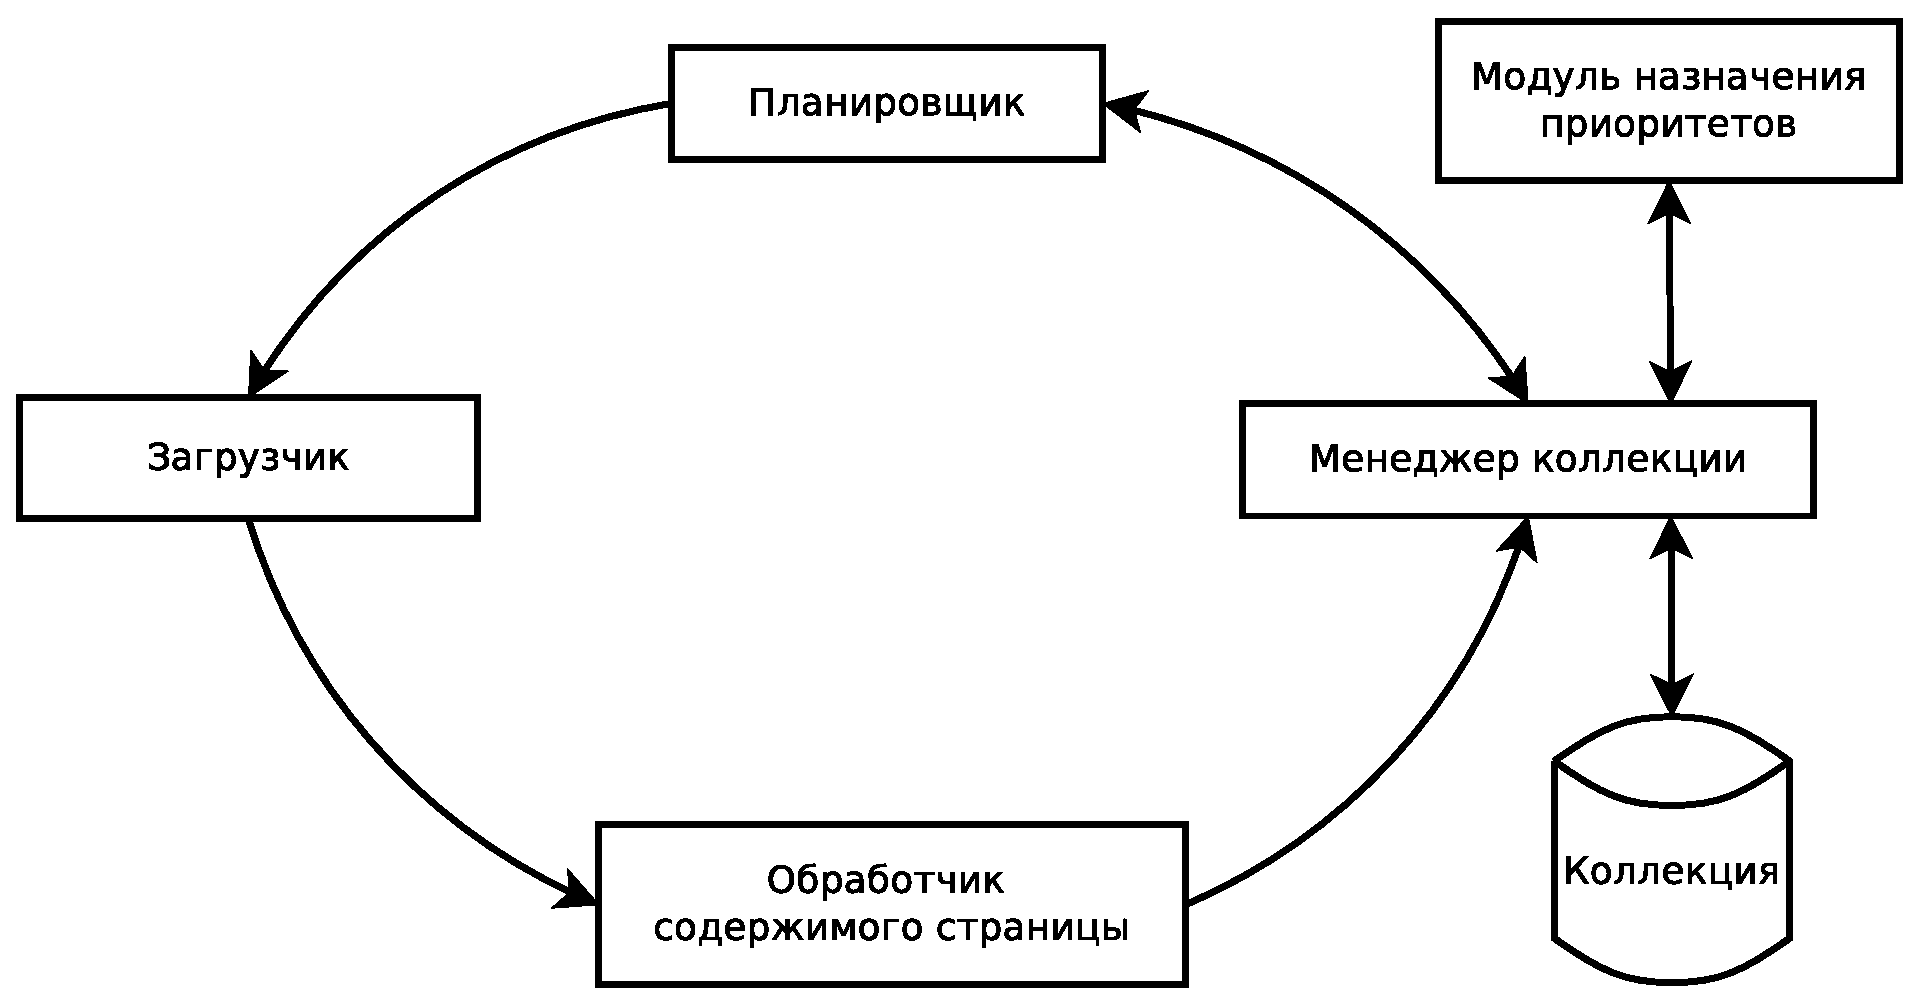
\includegraphics[width=1\linewidth]{pics/architecture.eps}}
\caption{Основные программные компоненты поискового робота}
\label{architecture}
\end{figure}

Алгоритм проходит включает в себя два этапа: подготовительный  и основной. На подготовительном этапе происходит инициализация модуля назначения приоритетов, а на основном --- непосредственно обход интернета. Рассмотрим подробнее каждый из этапов.

\subsection*{Подготовительный этап}

На подготовительном этапе происходит обучение нейронной сети, которая входит в модуль назначения приоритетов. В качестве обучающего множества используется набор URL-адресов веб-страниц с известными рангами (например, $PageRank$). Затем в коллекцию добавляется стартовое множество URL-адресов, и для каждого из них вычисляется $QRank$.

\subsection*{Основной этап}

Работа алгоритма на основном этапе происходит циклически. На каждом шаге цикла обрабатывается $K$ страниц из коллекции, имеющих наибольший $VRank$. 

Цикл начинается с того, что планировщик запрашивает у менеджера коллекции следующую партию адресов веб-страниц. После чего происходит подсчет $VRank$ для каждой страницы из коллекции посредством запросов менеджера коллекции к модулю приоритезации. Затем менеджер коллекции формирует партию, содержащую $K$ адресов веб-страниц, имеющих наибольший $VRank$ и передает ее планировщику. После чего планировщик последовательно передает URL-адреса для дальнейшей обработки. 

Обработка начинается с загрузки веб-страницы, получаемой по текущему URL-адресу. Следует помнить, что при загрузке следует учитывать правила вежливости, описанные в разделе \ref{spider}. И в любой момент времени с каждым хостом должно быть установлено не более одного соединения. После загрузки следует проверить, обновилась ли страница с момента предыдущего посещения, чтобы осуществить пересчет предполагаемого периода обновления для текущей страницы.

После чего обработчик содержимого страницы извлекает ссылки с загруженной. После чего из каждой ссылки извлекается URL-адрес. Полученное множество адресов передается менеджеру коллекции. После чего происходит расчет $QRank$ для каждого URL-адреса, извлеченного с текущей страницы. Расчет производит модуль приоритезации.

Когда все $K$ страниц из текущей партии будут обработаны, алгоритм перейдет к следующему шагу цикла.

\section{Статические особенности URL-адреса}
\label{static_features}

Для вычисления $QRank$ веб-страницы были использованы следующие статические особенности ее URL-адреса. Они были разделены на четыре группы.

\subsection*{Особенности длины}

В эту группу включены особенности, характеризующие длины компонент URL-адреса. Такие как:

\begin{itemize}
\item Суммарное число символов URL-адреса;
\item Число символов схемы URL-адреса;
\item Число символов хоста;
\item Число символов пути;
\item Число символов запроса.
\end{itemize}

\subsection*{Орфографические особенности}

В эту группу включены особенности, характеризующие орфографические свойства URL-адреса и его компонент. Такие как:

\begin{itemize}
\item Суммарное число цифр, входящих в URL-адрес;
\item Суммарное число заглавных букв, входящих в URL-адрес;
\item Число цифр, содержащихся в хосте;
\item Число цифр, содержащихся в пути URL-адреса;
\item Число цифр, содержащихся в запросе URL-адреса;
\item Число заглавных букв, содержащихся в пути URL-адреса;
\item Число заглавных букв, содержащихся в запросе URL-адреса.
\end{itemize}

\subsection*{Количественные особенности термов}

В данную группу включены особенности, характезующие количество термов в URL-адресе и его компонентах. Разделение на термы осуществлялось посредством разбиения адреса по символом, не являющимися буквами или цифрами. После чего выделялись следующие особенности:

\begin{itemize}
\item Суммарное число термов URL-адреса;
\item Число термов хоста;
\item Число термов пути;
\item Число термов запроса.
\end{itemize}

\subsection*{Словарные особенности термов}

В эту группу включены компоненты, характеризующие частоту реальных слов в компонентах URL-адреса. А именно:

\begin{itemize}
\item Частота реальных слов среди термов, входящих в путь URL-адреса;
\item Частота реальных слов среди термов, входящих в запрос.
\end{itemize}

\chapter{Экспериментальные результаты}
\label{chapter_experiment}

Предлагаемый метод был реализован в виде программной системы на языке \textit{Java} и протестирован.

\section{Реализация}

При реализации предлагаемого метода были реализованы следующие программные компоненты:
\begin{itemize}
\item Обертка для URL-адреса;
\item Менеджер хоста;
\item Модуль вежливости;
\item Правило;
\item Планировщик;
\item Задание;
\item Загрузчик веб-страниц;
\item Обработчик содержимого страницы;
\item Модули назначения приоритетов:
\begin{itemize}
\item Стратегия обхода в ширину;
\item Использующий нейронную сеть;
\item Использующиуй нейронную сеть и свойства веб-графа;
\end{itemize}
\item Контроллер приоритезации, использующей нейронную сеть;
\item Компонент для извлечения особенностей URL-адреса страницы;
\item Компонент, содержащий нейронную сеть;
\item Словарный модуль;
\item Менеджер коллекции.
\end{itemize}

Основным объектом, с которым происходит работа в программе, является обертка для URL-адреса. Она реализована классом \textit{WebURL}. Каждый экземпляр такого класса содержит мета-информацию о веб-странице, ее $QRank$, время последнего посещения, предполагаемый период обновления, ссылку на менеджер хоста и т.д.

Менеджер хоста  реализован классом \textit{HostController} и предназначен для выполнения правил вежливости для определенного хоста. В каждый момент времени с хостом должно быть установлено только одно соединение. Это реализовано за счет синхронизирования загрузок веб-страницы с одного хоста посредством использования поля \textit{lock} менеджера хоста, являющегося экземпляром класса \textit{Lock}. Кроме того, экземляр класса хранит на модуль вежливости, который определяет правила доступа к страницам хоста. Также менеджер хранит количество страниц с текущего хоста, имеющихся в коллекции.

Модуль вежливости предназначен для соблюдения правил вежливости, описанных в файле \textit{robots.txt}, содержащемуся в корневом каталоге многих сайтов. Модуль вежливости реализован классом \textit{PolitenessModule}, содержащий множество (экземляр класса \textit{TreeSet}) правил, являющихся экземплярами класса \textit{Rule}. Правило хранит текстовый шаблон (\textit{Pattern}), удовлетворяющий набору каталогов сайта, и правило доступа (доступно или нет). Порядок на множестве введен для быстрого определения доступности того или иного URL-адреса.

Планировщик реализован классом \textit{Scheduler}. Планировщик на каждом шаге цикла основного этапа алгоритма формирует $K$ заданий, являющихся экземплярами исполняемого (\textit{Runnuble}) класса \textit{PageProceccingTask}. Эти задания передаются исполнителю (экземпляр класса \textit{ExecutorService}). Задание состоит из следующих инструкций для последовательной обработки. Загрузка, осуществляемая загрузчиком веб-страниц. Обработка содержимого и извлечение ссылок со страницы, осуществляемые обаботчиком содержимого страницы. И наконец отправка менеджеру коллекции для дальнейшей обработки. Обработка заданий осуществляется в несколько потоков.

Модуль назначения приоритетов является экземпляром класса, наследующего абстрактный класс \textit{PrioritizationModule}. Разработаны два метода приоритезации: первый использует только нейронную сеть, а второй --- нейронную сеть и анализ веб-графа. Реализованы они соотвественно классами \textit{NeuralPrioritizationModule} \textit{NeuralGraphPrioritizationModule}, исходный код которых приведен в приложениях: \ref{code_1} и \ref{code_2}. Кроме того, были реализованы методы приоритезации: \textit{breadth-first}, реализующий стратегию отбора методом обхода в ширину, и \textit{Random},  для сравнения с разработанными стратегиями приоритезации.

Компонент для извлечения особенностей URL-адреса реализован классом \textit{FeaturesExtractor}. Исходный программный код класса приведен в приложении \ref{code_3}. Для каждой из особенностей адреса компонент реализует его численное представление в интервале от $0$ до $1$ посредством нормировки. Для извлечения словарных особенностей термов конструируется словарный модуль, использующий слова английского и русского языков. Причем слова русского языка были заменены на их транслитерационный вид.

Нейронная сеть была реализована с использованием библиотеки \textit{Encog} \cite{encog}. Сеть содержит три слоя нейронов. Входной слой содержит число нейронов, соответствующее числу особенностей URL-адреса веб-страницы (максимальное число особенностей --- $16$). Слой имеет сигмоидную активирующую функцию. Число нейронов в скрытом слое зависит от числа нейронов входного слоя. А именно --- число нейронов скрытого слоя в три раза больше. Скрытый слой так же имеет сигмоидную активирующую функцию. Выходной слой содержит один нейрон и сигмоидную активирующую функцию. Для обучения использовался метод быстрого распространения (\textit{Quickprop}), являющийся улучшением метода обратного распространения ошибки. Подробно он описан в статье \cite{Fahlman88anempirical}. Данная конфигурация сети была подобрана в ходе тестирования на множестве URL-адресов веб-страниц с известными $PageRank$, полученными с использованием \textit{google toolbar}. Именно с такими параметрами отклонение вычисленного ранга от реального $PageRank$ было минимальным.

Менеджер коллекции реализован классом \textit{CollectionHandler}. Он содержит ссылку на модуль приоритезации, посредством которого вычисляются ранги для URL-адресов веб-страниц, передаваемых в коллекцию. Коллекция представлена экзампляром класса \textit{ConcurrentHashMap}, где ключом является строка, а значением --- \textit{WebURL}. Выбрана потоко-безопасная реализация ассоциативного массива, поскольку добавление адресов происходит в несколько потоков. Также менеджер коллекции содержит множество менеджеров хостов для того, чтобы контролировать количество добавляемых в коллекцию страниц. Кроме того, менеджер коллекции осуществляет формирования пакета веб-страниц для обработки по запросу планировщика. Формирование осуществляется путем подсчета $VRank$ для каждой страницы коллекции и выбора $K$ страниц с наибольшим таким рангом. Для эффективной реализации такой сортировки был реализован компаратор \textit{ValueComparator}, осуществляющий сортировку в \textit{Map} по значению. В процессе формирования партии веб-страниц контролируется, чтобы она не содержала более определенного в планировщике числа страниц с одного сайта. Это необходимо для того, чтобы поисковый робот не зацикливался на одном сайте, что привело бы к замедлению работы.

\section{Параметры запусков}

Для сравнения работы различных стратегий приоритезации были произведены тестовые запуски поискового робота на сайтах, принадлежищих домену \textit{.ru}. Стартовое множество URL-адресов состояло из главных страниц ста популярных сайтов, принадлежащих тому же домену. 
Максимальное число обрабатываемых сайтов составляло $5000$, при этом с каждого сайта обрабатывалось не более $500$ страниц. Размер партии страниц, обрабатываемых на одной итерации цикла составляло $K = 1000$, причем максимальное число страниц с одного сайта в ней составяло $50$. Обработка страниц происходила в $20$ параллельных потоков.

Нейронная сеть была обучена на случайной выборке размером $50000$ URL-адресов с домена \textit{.ru}, для которых были известны их $PageRank$, полученные посредством использования веб-сервиса $Google Toolbar$, за счет осуществления запросов к $toolbarqueries.google.com$. Данный сервис по URL-адресу страницы возращает целое число из отрезка от $-1$ до $10$, являющееся $Google PageRank$ данной страницы, то есть оценкой важности страницы по мнению $Google$, которое вследствие линейной нормировки приводилось к действительному числу из отрезка от $0$ до $1$.

\section{Результаты}

Были протестированы стратегии приоритезации, реализующие два предложенных метода, стратегия, использующая обход в ширину, а также стратегия, при которой страницы из очереди выбирались случайным образом с равными вероятностями. В процессе обхода интернета при каждом запуске в коллецию добавлялось около $200$ тысяч URL-адресов, из которых были скачаны $25$ тысяч страниц с адресами, имеющими наибольший приоритет. Для всех скачанных в процессе запусков страниц был получен их $PageRank$ с использованием сервиса $Google Toolbar$, являющийся показателем их качества. На рисунке \ref{graphic} приведен график завимости среднего $PageRank$ страниц от числа скачанных для каждой из протестированных стратегий приортезации.

\begin{figure}[h!]
\center{\includegraphics[width=1\linewidth]{pics/ranges5.png}}
\caption{График зависимости среднего $PageRank$ страниц от скачанного числа страниц. $BFS$ --- стратегия обхода в ширину. $Neural$ --- стратегия приоритезации, использующая нейронную сеть. $Neural + Graph$ --- стратегия приоритезации использующая нейронную сеть и веб-граф. $Random$ --- стратегия приоритезации, случайно выбирающая из коллекции страницу для скачивания.}
\label{graphic}
\end{figure}

Соответственно, стратегия тем лучше, чем выше $PageRank$ страниц, скачанных в процессе обхода интернета поисковым роботом, использующим ее, то есть, чем выше линия на графике.

\section{Выводы}

Полученные результаты экспериментального сравнения позволяют сделать следующие выводы:

\begin{enumerate}
\item Стратегия приоритезации, использующая метод обхода в ширину, превосходит стратегию, случайно выбирающую страницы.
\item Предложенные в работе стратегии приоритезации поискового робота, превосходят стандартную стратегию обхода в ширину.
\item Результаты обхода интернета с использованием двух предложенных стратегий отличаются незначительно.
\end{enumerate}


\startconclusionpage

В работе получены следующие результаты. Предложены и разработаны две стратегии приоритезации поискового робота, использующие статические признаки URL-адресов. 

Тестовые запуски показали, что поисковый робот, использующий любую из них, скачивает более качественные страницы, чем поисковый робот, использующий обход в ширину.

\bibliography{thesis}

\startappendices
\chapter{Программный код}

\section{Программный код модуля модуля назначения приоритетов, использующего нейронную сеть}
\label{code_1}

\lstset{ %
  language=Java,                % the language of the code
  basicstyle=\small,           % the size of the fonts that are used for the code
  numbers=left,                   % where to put the line-numbers
  numberstyle=\tiny\color{gray},  % the style that is used for the line-numbers
  stepnumber=2,                   % the step between two line-numbers. If it's 1, each line 
                                  % will be numbered
  numbersep=5pt,                  % how far the line-numbers are from the code
  backgroundcolor=\color{white},      % choose the background color. You must add \usepackage{color}
  showspaces=false,               % show spaces adding particular underscores
  showstringspaces=false,         % underline spaces within strings
  showtabs=false,                 % show tabs within strings adding particular underscores
  frame=none,                   % adds a frame around the code
  rulecolor=\color{black},        % if not set, the frame-color may be changed on line-breaks within not-black text (e.g. commens (green here))
  tabsize=2,                      % sets default tabsize to 2 spaces
  captionpos=b,                   % sets the caption-position to bottom
  breaklines=true,                % sets automatic line breaking
  breakatwhitespace=false,        % sets if automatic breaks should only happen at whitespace
 % title=\lstname,                   % show the filename of files included with \lstinputlisting;
                                  % also try caption instead of title
  keywordstyle=\color{blue},          % keyword style
  commentstyle=\color{dkgreen},       % comment style
  stringstyle=\color{mauve},         % string literal style
  escapeinside={\%*}{*)},            % if you want to add a comment within your code
  morekeywords={*,...}               % if you want to add more keywords to the set
}


\lstinputlisting[language=Java,caption={Модуль назначения приоритетов, использующий нейронную сеть}]
{/home/nastik/workspace/crawler/src/main/java/ru/ifmo/mailru/priority/NeuralPrioritizationModule.java}
\section{Программный код модуля модуля назначения приоритетов, использующего нейронную сеть и свойства веб-графа}
\label{code_2}
\lstinputlisting[language=Java,caption={Модуль назначения приоритетов, использующий нейронную сеть и свойства веб-графа}]{/home/nastik/workspace/crawler/src/main/java/ru/ifmo/mailru/priority/NeuralGraphPrioritizationModule.java}

\section{Программный код модуля выделения статических особенностей URL-адреса}
\label{code_3}
\lstinputlisting[language=Java,caption={Модуль выделения статических особенностей URL-адреса}]{//home/nastik/workspace/crawler/src/main/java/ru/ifmo/mailru/features/FeaturesExtractor.java}

\end{document}
